%% using aastex version 6.3
\documentclass[twocolumn]{aastex63}

\newcommand{\vdag}{(v)^\dagger}
\newcommand\aastex{AAS\TeX}
\newcommand\latex{La\TeX}

%%%%%%%%%%%%%%%%%%%%%%%%%%%%%%%%%%%%%%%%%%%%%%%%%%%%%%%%%%%%%%%%%%%%%%%%%%%%%%%%
%%
%% The following section defines new commands for comments from co-authors
%%
\definecolor{DarkOrange}{RGB}{204, 85, 0}
\definecolor{LincolnGreen}{RGB}{17, 102, 0}
\definecolor{Rust}{HTML}{9B4F0F}
\definecolor{Blueberry}{HTML}{063852}

\def\ion#1#2{#1$\;${\footnotesize\rm{#2}}\relax}

\newcommand{\kate}[1]{{\color{red} KM: {#1}}}
\newcommand{\fromkate}[1]{{\color{brown} fromKM: {#1}}}
\newcommand{\steve}[1]{{\color{Blueberry} Steve S: {#1}}}
\newcommand{\magee}[1]{{\color{Rust} MM: {#1}}}

\newcommand{\abi}[1]{{\color{LincolnGreen} AP: {#1}}}
\newcommand{\yy}[1]{{\color{blue} YY: {#1}}}
\newcommand{\aam}[1]{{\color{DarkOrange} aam: {#1}}}
\newcommand{\stockholm}[1]{{\color{cyan} stockholm: {#1}}}
\newcommand{\todo}[1]{{\color{magenta} to-do: {#1}}}

\newcommand{\rztf}{$r_\mathrm{ZTF}$}
\newcommand{\gztf}{$g_\mathrm{ZTF}$}
\newcommand{\iztf}{$i_\mathrm{ZTF}$}
\newcommand{\tfl}{$t_\mathrm{fl}$}
\newcommand{\trise}{$t_\mathrm{rise}$}
\newcommand{\tbmax}{$T_{B,\mathrm{max}}$}
\newcommand{\kms}{km\,s$^{-1}$}
\newcommand{\RSiII}{$\mathcal{R}($\ion{Si}{II}$)$}
\newcommand{\radni}{$^{56}$Ni}

\newcommand{\sn}{SN\,2019yvq}

%%
%%%%%%%%%%%%%%%%%%%%%%%%%%%%%%%%%%%%%%%%%%%%%%%%%%%%%%%%%%%%%%%%%%%%%%%%%%%%%%%%

%% Reintroduced the \received and \accepted commands from AASTeX v5.2
\received{\today}
\revised{}
\accepted{}
%% Command to document which AAS Journal the manuscript was submitted to.
%% Adds "Submitted to " the argument.
\submitjournal{ApJ}

%% For manuscript that include authors in collaborations, AASTeX v6.3
%% builds on the \collaboration command to allow greater freedom to 
%% keep the traditional author+affiliation information but only show
%% subsets. The \collaboration command now must appear AFTER the group
%% of authors in the collaboration and it takes TWO arguments. The last
%% is still the collaboration identifier. The text given in this
%% argument is what will be shown in the manuscript. The first argument
%% is the number of author above the \collaboration command to show with
%% the collaboration text. If there are authors that are not part of any
%% collaboration the \nocollaboration command is used. This command takes
%% one argument which is also the number of authors above to show. A
%% dashed line is shown to indicate no collaboration. This example manuscript
%% shows how these commands work to display specific set of authors 
%% on the front page.
%%
%% For manuscript without any need to use \collaboration the 
%% \AuthorCollaborationLimit command from v6.2 can still be used to 
%% show a subset of authors.
%
%\AuthorCollaborationLimit=2
%
%% will only show Schwarz & Muench on the front page of the manuscript
%% (assuming the \collaboration and \nocollaboration commands are
%% commented out).
%%
%% Note that all of the author will be shown in the published article.
%% This feature is meant to be used prior to acceptance to make the
%% front end of a long author article more manageable. Please do not use
%% this functionality for manuscripts with less than 20 authors. Conversely,
%% please do use this when the number of authors exceeds 40.
%%
%% Use \allauthors at the manuscript end to show the full author list.
%% This command should only be used with \AuthorCollaborationLimit is used.

%% The following command can be used to set the latex table counters.  It
%% is needed in this document because it uses a mix of latex tabular and
%% AASTeX deluxetables.  In general it should not be needed.
%\setcounter{table}{1}

%%%%%%%%%%%%%%%%%%%%%%%%%%%%%%%%%%%%%%%%%%%%%%%%%%%%%%%%%%%%%%%%%%%%%%%%%%%%%%%%
%%
%% The following section outlines numerous optional output that
%% can be displayed in the front matter or as running meta-data.
%%
%% If you wish, you may supply running head information, although
%% this information may be modified by the editorial offices.
\shorttitle{\sn\ is Fun and Cool}
\shortauthors{Miller et al.}
%%
%% You can add a light gray and diagonal water-mark to the first page 
%% with this command:
\watermark{DRAFT}
%% where "text", e.g. DRAFT, is the text to appear.  If the text is 
%% long you can control the water-mark size with:
%% \setwatermarkfontsize{dimension}
%% where dimension is any recognized LaTeX dimension, e.g. pt, in, etc.
%%
%%%%%%%%%%%%%%%%%%%%%%%%%%%%%%%%%%%%%%%%%%%%%%%%%%%%%%%%%%%%%%%%%%%%%%%%%%%%%%%%
\graphicspath{{./}{figures/}}
%% This is the end of the preamble.  Indicate the beginning of the
%% manuscript itself with \begin{document}.

\begin{document}

\title{\sn\  }

%% LaTeX will automatically break titles if they run longer than
%% one line. However, you may use \\ to force a line break if
%% you desire. In v6.3 you can include a footnote in the title.

%% A significant change from earlier AASTEX versions is in the structure for 
%% calling author and affiliations. The change was necessary to implement 
%% auto-indexing of affiliations which prior was a manual process that could 
%% easily be tedious in large author manuscripts.
%%
%% The \author command is the same as before except it now takes an optional
%% argument which is the 16 digit ORCID. The syntax is:
%% \author[xxxx-xxxx-xxxx-xxxx]{Author Name}
%%
%% This will hyperlink the author name to the author's ORCID page. Note that
%% during compilation, LaTeX will do some limited checking of the format of
%% the ID to make sure it is valid. If the "orcid-ID.png" image file is 
%% present or in the LaTeX pathway, the OrcID icon will appear next to
%% the authors name.
%%
%% Use \affiliation for affiliation information. The old \affil is now aliased
%% to \affiliation. AASTeX v6.3 will automatically index these in the header.
%% When a duplicate is found its index will be the same as its previous entry.
%%
%% Note that \altaffilmark and \altaffiltext have been removed and thus 
%% can not be used to document secondary affiliations. If they are used latex
%% will issue a specific error message and quit. Please use multiple 
%% \affiliation calls for to document more than one affiliation.
%%
%% The new \altaffiliation can be used to indicate some secondary information
%% such as fellowships. This command produces a non-numeric footnote that is
%% set away from the numeric \affiliation footnotes.  NOTE that if an
%% \altaffiliation command is used it must come BEFORE the \affiliation call,
%% right after the \author command, in order to place the footnotes in
%% the proper location.
%%
%% Use \email to set provide email addresses. Each \email will appear on its
%% own line so you can put multiple email address in one \email call. A new
%% \correspondingauthor command is available in V6.3 to identify the
%% corresponding author of the manuscript. It is the author's responsibility
%% to make sure this name is also in the author list.
%%
%% While authors can be grouped inside the same \author and \affiliation
%% commands it is better to have a single author for each. This allows for
%% one to exploit all the new benefits and should make book-keeping easier.
%%
%% If done correctly the peer review system will be able to
%% automatically put the author and affiliation information from the manuscript
%% and save the corresponding author the trouble of entering it by hand.

% \author[0000-0001-9515-478X]{A.~A.~Miller}
% \affiliation{Center for Interdisciplinary Exploration and Research in Astrophysics (CIERA) and Department of Physics and Astronomy, Northwestern University, 2145 Sheridan Road, Evanston, IL 60208, USA}
% \affiliation{The Adler Planetarium, Chicago, IL 60605, USA}
% \email{amiller@northwestern.edu}

\author{ZTF}

\author{et al.}

%% Note that the \and command from previous versions of AASTeX is now
%% depreciated in this version as it is no longer necessary. AASTeX 
%% automatically takes care of all commas and "and"s between authors names.

%% Mark off the abstract in the ``abstract'' environment. 
\begin{abstract}

\todo{Write the abstract}

\end{abstract}

%% Keywords should appear after the \end{abstract} command. 
%% See the online documentation for the full list of available subject
%% keywords and the rules for their use.
\keywords{}

\section{Introduction} \label{sec:intro}

\todo{write it; define and include references for ZTF}

\section{Discovery and Observations}\label{sec:obs}

\sn\ was discovered by K.~Itagaki, and detected at an unfiltered magnitude of
16.7\,mag, in an image obtained on 2019 Dec 28.74 UT\footnote{UT times are
used throughout this paper}. The transient candidate was announced
$\sim$2\,hr later on the Transient Name Server (TNS), and given the
designation AT\,2019yvq \citep{Itagaki19}. Susequent spectroscopic
observations confirmed the SN nature of the transient, with initial reports
that the event was a SN Ib/c \citep{Kawabata20}, but later reports classified
the event as a SN Ia \todo{create refs for Prentice obs}. These spectroscopic
observations also showed \sn\ to be at the same redshift as NGC\,4441, its
host galaxy.

\subsection{ZTF Photometric Observations}

ZTF simulataneously conducts multiple time-domain surveys using the ZTF
camera on the the Palomar Oschin Schmidt 48 inch (P48) telescope. \sn\ was
first detected by ZTF on 2019 Dec 29.46, as part of the ZTF public survey
(see \citealt{Bellm19a}). The automated ZTF pipeline \citep{Masci19}
automatically detected \sn, which passed internal thresholds (e.g.,
\citealt{Mahabal19}), leading to the production and disemination of a
real-time alert \citep{Patterson19}. The public alert included the position,
$\alpha = 12^{\mathrm{h}}27\arcmin21\farcs836$, $\delta =
+64\degr47\arcmin59\farcs87$ (J2000), and brightness, \rztf$ =
17.14\pm0.05$\,mag, which, together with the \citet{Itagaki19} discovery
report suggested the SN was fading. Continued monitoring with ZTF, and
follow-up with other telescopes, confirmed a spectacular decline in the early
emission from \sn\ (Figure~\ref{fig:p48}).

\begin{figure*}
    \centering
    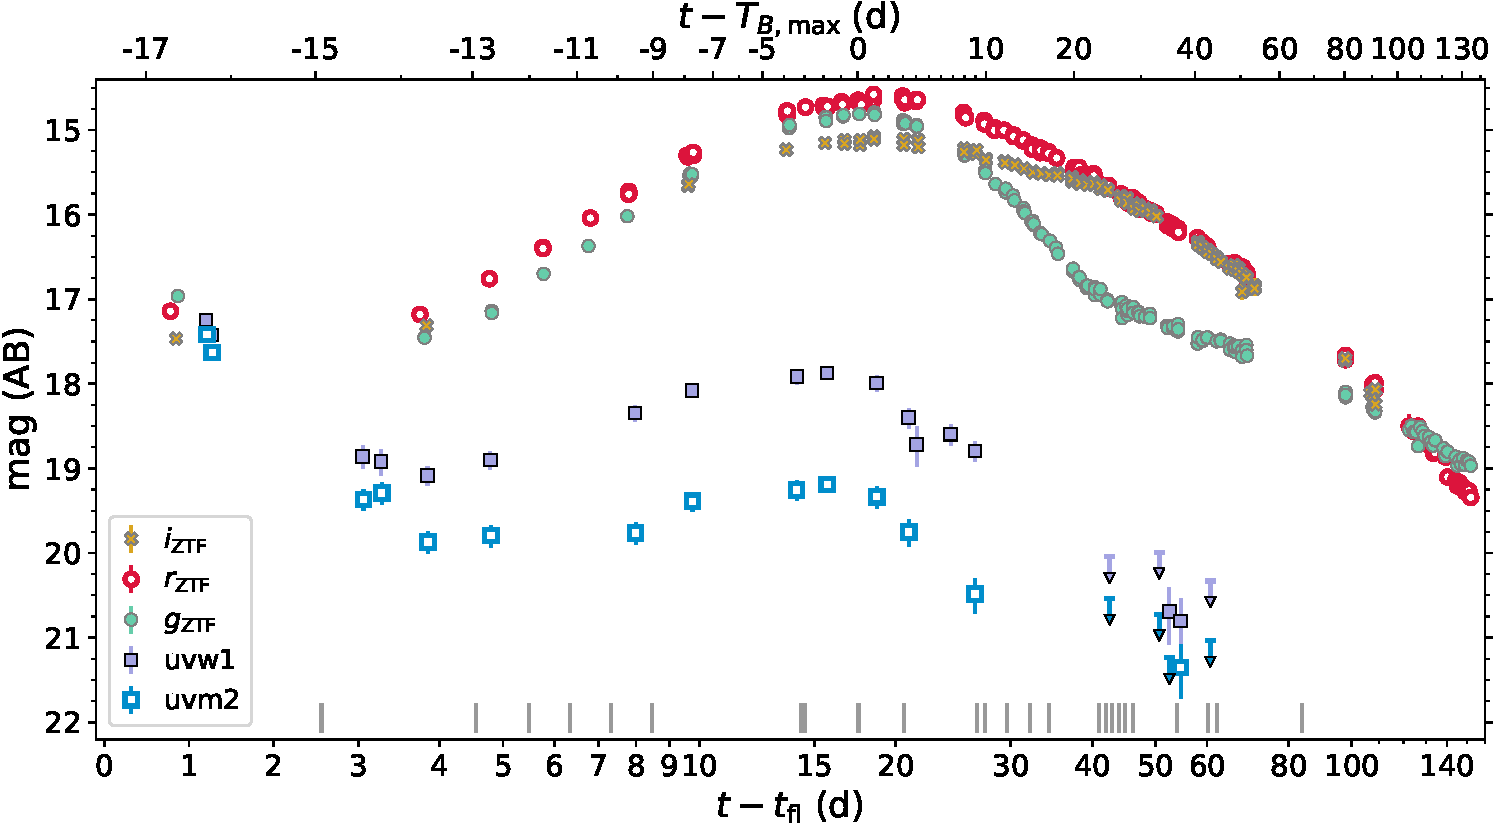
\includegraphics[width=6in]{./figures/P48_lc.pdf}
    %
    \caption{Photometric evolution of \sn, highlighting the initial decline
    observed in the light curve. \gztf, \rztf, and \iztf\ observations are
    shown as filled green circles, open red circles, and filled golden
    crosses, respectively. UVOT $uvw1$ and $uvm2$ are shown as filled and
    open squares, respectively. The lower axis shows time measured in
    rest-frame days relative to the time of first light, \tfl (see
    \S\ref{sec:phot}), while the upper axis shows time relative to the time
    of $B$-band maximum, \tbmax. Note that the horizontal axis is shown with
    a linear scale from $0\,\mathrm{d} \le t - t_\mathrm{fl} \le 3$\,d and a
    log scale for $t - t_\mathrm{fl} > 3$\,d. Vertical grey ticks show
    epochs of spectroscopic observations.}
    %
    \label{fig:p48}
\end{figure*}

The field of \sn\ was additionally observed by ZTF with nearly a nightly
cadence as part of the ZTF partnership Uniform Depth Survey (ZUDS;
D.~Goldstein et al., in prep.). Using images obtained as part of the ZUDS
program, we perform forced PSF photometry at the location of \sn\ following
the procedure described in \citet{Yao19}.\footnote{Images obtained as part of
the ZTF public survey have not been released, preventing us from applying our
forced-PSF measurements. We therefore only include forced-PSF measurements in
the analysis described herein, though we note that our measurements are
largely consistent with those provided in the public alerts.} The evolution
of \sn\ in the \gztf, \rztf, and \iztf\ filters is shown in
Figure~\ref{fig:p48}.

\subsection{Other Photometric Observations}

Ultraviolet (UV) observations of \sn\ were obtained with the
Ultra-Violet/Optical Telescope (UVOT; \citet{Roming05}) onboard the Neil
Gehrels Swift Observatory (hereafter \textit{Swift}; \citealt{Gehrels04})
following a time-of-opportunity request.\footnote{\textit{Swift} ToO requests
for \sn\ (\textit{Swift} Target ID: 13037) have been submitted by
D.~Hiramatsu, Burke \todo{what is Burke's first initial?}, and S.~Schulze.}
Pre-SN UVOT reference images are limited to the $uvw1$, $uvm2$, and $uvw2$
filters. We estimate the flux in these filters using an aperture of size
\steve{PPP} pixels at the SN position, and subtract the flux measured using
an identical procedure in the pre-SN images \steve{Is this all correct?}. For
clarity, we only show the \textit{Swift} $uvw1$ and $uvm2$ light curves in
Figure~\ref{fig:p48} (the $uvw2$ evolution is nearly identical to $uvm2$).
\textit{Swift}/UVOT observations show that the initial decline seen in the
optical is even more dramatic in the UV.

While we exclude flux measurements in the UVOT $u$, $b$, and $v$ filters in
our analysis below, we can nevertheless estimate the time of $B$-band maximum
\tbmax\ from the host-contaminated $b$-band light curve given that the host
flux provides a constant offset at all epochs. Using a second-order
polynomial, we model the $b$-band light curve near peak (including
observations between JD$\,> \,$2,458,855.5 and JD$\,<\,$2,458,871.5). From
this fit we estimate \tbmax$ = $2,458,863.83$ \,\pm \,0.21$\,JD.

\todo{add paragraph about X-ray limits}

\subsection{Optical Spectroscopy}

Spectroscopic observations of \sn\ were taken with a variety of telescopes
and instruments over multiple epochs beginning $\sim$3\,d after discovery and
continuing through $\sim$7\,wk after \tbmax \todo{update these numbers}. An
observing log is listed in Table~\ref{tab:spectra}. The spectra were reduced
using standard procedures in \texttt{IDL}/\texttt{Python}/\texttt{Matlab}.
The optical spectral evolution of \sn\ is illustrated in
Figure~\ref{fig:spec_evo}.

\begin{figure}
    \centering
    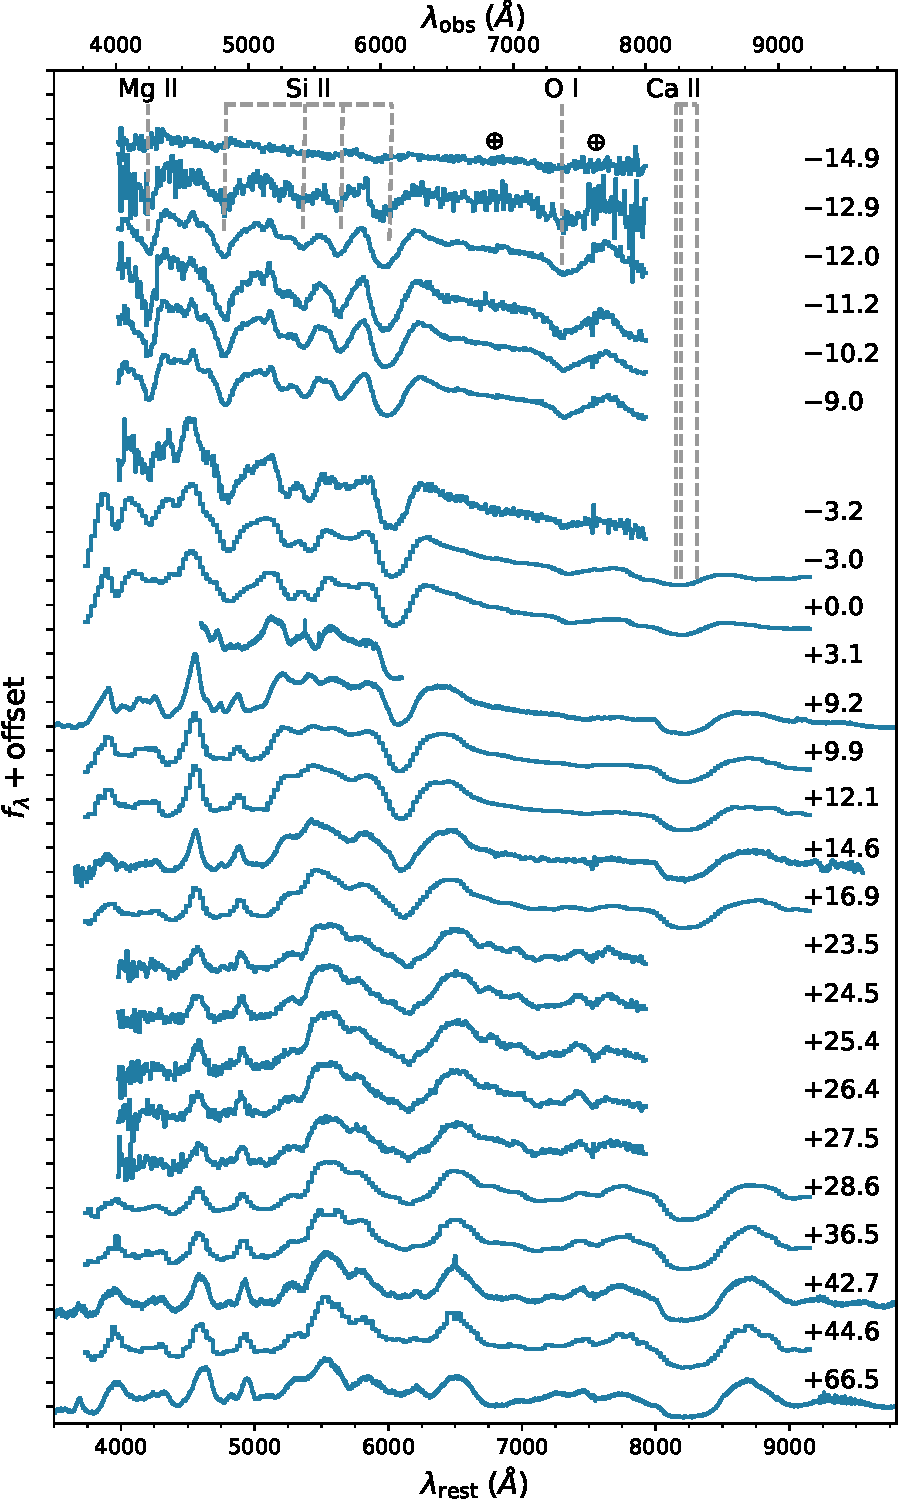
\includegraphics[width=3.35in]{./figures/spec_evo.pdf}
    %
    \caption{Observed spectral sequence of \sn. Spectra have been normalized
    by their median flux between 7200\,\AA\ and 7400\,\AA. The phase of each
    observation relative to \tbmax\ is shown to the right of the individual
    spectra. Prominent spectral features from intermediate mass elements are
    highlighted with vertical dashed lines. Some of the spectra show
    imperfect Telluric subtractions, giving rise to the non-smooth features
    around $\lambda_\mathrm{obs} \approx 7600$\,\AA.}
    %
    \label{fig:spec_evo}
\end{figure}


\section{Analysis}\label{sec:analysis}

\subsection{NGC\,4441: the Host of \sn}\label{sec:host}

NGC\,4441 is the host galaxy of \sn. SDSS spectroscopic measurements of the
nucleus of NGC\,4441 yield a heliocentric-recession velocity of 2663\,\kms\
($z_\mathrm{helio} = 0.00888$; \citealt{Abolfathi18}) and a \texttt{STARBURST}
classification for NGC\,4441. Using the 2M++ model of \citet{Carrick15}, we
estimate a peculiar velocity towards NGC\,4441 of $+328.6$\,\kms, which
combined with the recession velocity in the frame of the cosmic microwave
background\footnote{See
\url{https://ned.ipac.caltech.edu/velocity_calculator}} (CMB, $v_\mathrm{CMB}
= 2770$\,\kms), yields a total recession velocity $\approx 3100$\,\kms. We
note that this estimate is consistent, to within $\sim$5\%, with the Virgo and
Great Attractor infall models of \citet{Mould00}. Adopting $H_0 =
73$\,\kms\,Mpc$^{-1}$, we estimate the distance to NGC\,4441 to be 42.5\,Mpc,
corresponding to a distance modulus of $\mu = 33.14 \pm 0.15$\,mag, where the
uncertainty on $\mu$ is dominated by the uncertainty in the peculiar velocity
correction. We hereafter adopt 33.14\,mag as the distance modulus to
NGC\,4441.\footnote{\citet{Tonry01} estimate a significantly smaller distance
to NGC\,4441 ($\mu = 31.40 \pm 0.45$\,mag; $D = 19.0$\,Mpc) based on surface
brightness fluctuations (SBF). We do not adopt this estimate as SBF
measurements are better suited to relative distance measurements.} \todo{Lots
of differrent catalogs provide metallicity for SDSS galaxies, should we report
on these results at all? Port Z = 0.04 and Granada Z ~0.01, and do not agree,
firefly ~ 0.6 0r 0.2 (solar?) depending on weighting, probably not a great
idea}

We estimate the total redenning towards \sn\ to be small. There is relatively
little line of sight extinction due to the Milky Way, $E(B-V) \approx
0.018$\,mag \citep{Schlafly11, Schlegel98}. Furthermore, we do not find
significant evidence for strong extinction in NGC\,4441. Figure~\ref{fig:NaD}
highlights the \ion{Na}{I} D absorption in the spectrum of \sn\ due to gas in
NGC\,4441 and the Milky Way from our highest-resolution spectrum, $R \approx
4000$, obtained with Binospec+MMT. The \ion{Na}{I} D absorption is weak, and
we estimate a total equivalent width (EW) $= 390$\,m\AA\ for NGC\,4441 and
$220$\,m\AA\ for the Milky Way. There is a systematic uncertainty of
$\sim$10\% on each of these estimates due to uncertainties in the
continuum-fitting procedure. Assuming similar properties for the dust in
NGC\,4441 and the Milky Way, we scale the color excess measurement for the
Milky Way by the ratio of \ion{Na}{I} D EWs to estimate $E(B-V) \approx
0.032$\,mag for \sn\ due to absorption in NGC\,4441. This yields a total
color excess towards \sn\ of $E(B-V) \approx 0.05$\,mag, which we adopt for
the subsequent analysis in this study. We note that this estimate is
consistent, to within the uncertainties, with the EW(\ion{Na}{I} D)--$E(B-V)$
relations presented in \citet{Poznanski12}. Further supporting the claim of
low extinction is the lack of a detection of the \ion{K}{I}
$\lambda\lambda$7665, 7699 interstellar lines or the diffuse interstellar
band at 5780\,\AA, which also serve as proxies for extinction (e.g.,
\citealt{Phillips13}).

\begin{figure}
    \centering
    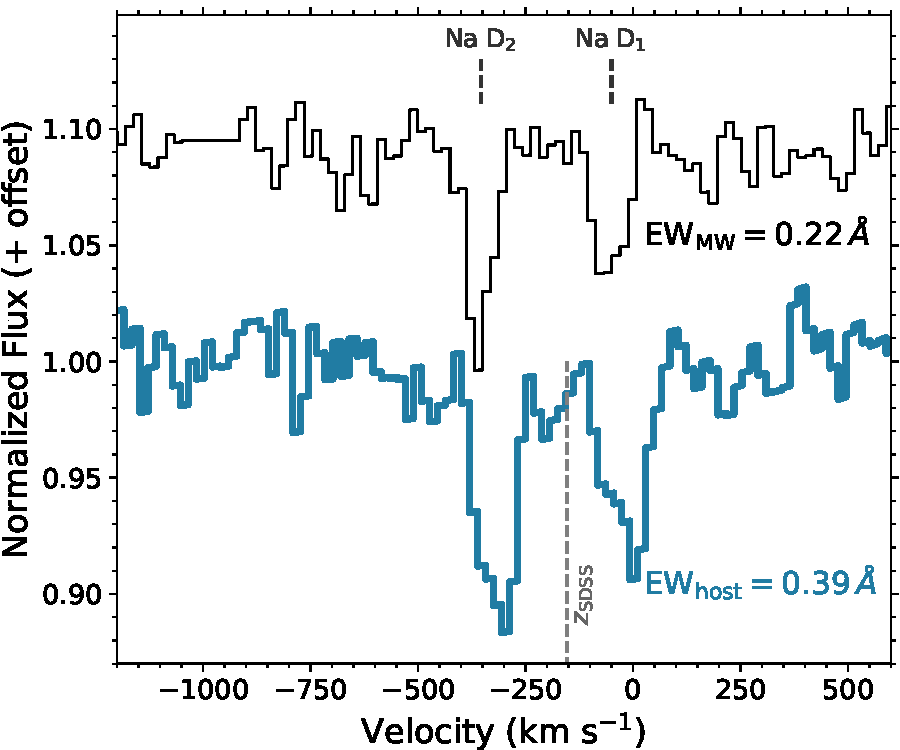
\includegraphics[width=3.35in]{./figures/NaD.pdf}
    %
    \caption{Zoom-in on our moderate resolution ($R \approx 4000$)
    MMT+Binospec spectrum of \sn\ highlighting absoprtion due to \ion{Na}{I}
    D in the host galaxy, NGC\,4441 (blue solid line), and the Milky Way
    (thin black line). The velocity scale is centered on the D$_1$ line in
    NGC\,4441, with the SDSS redshift shown via the vertical dashed line. No
    shift has been applied to the Milky Way lines. The \ion{Na}{I} D lines,
    which serve as a proxy for dust-obscuration along the line of sight
    (e.g., \citealt{Poznanski12,Phillips13}) are weak, indicating a
    relatively small amount of reddening.}
    %
    \label{fig:NaD}
\end{figure}



\subsection{Photometric Analysis}\label{sec:phot}

We estimate the time of first light, \tfl, for \sn\ following the procedure
described in \citet{Miller20}. Briefly, \citet{Miller20} model the early
emission from a SN Ia as a power-law in time, $f \propto (t -
t_\mathrm{fl})^\alpha$, where $f$ is the flux, $t$ is time, and $\alpha$ is
the power-law index. \tfl\ is assumed to be the same everywhere in the
optical, allowing us to simultaneously fit observations in each of the ZTF
filters.

An important caveat for \sn\ is that the observed early decline in the light
curve clearly does not follow the simple power-law model, and thus these
observations must be masked when performing the fit. We conservatively
exclude observations from the first two nights of ZTF detection from the fit
(this choice is conservative as it is unclear when the mechanism that powers
the initial bump in \sn\ no longer significantly contributes to the flux in
the \gztf\ and \rztf\ filters). From the fit we find \tfl$ = -17.5
\pm^{1.0}_{1.3}$\,d relative to \tbmax. We know that the time of explosion
must be $< -17.4$\,d based on the discovery detection in \citealt{Itagaki19},
and, by definition $t_\mathrm{fl} \ge t_\mathrm{exp}$, meaning a portion of
the posterior distribution for our model cannot be correct. We also find
$\alpha_g = 2.15 \pm^{0.49}_{0.36}$ and $\alpha_g = 1.91 \pm^{0.42}_{0.31}$.
These values are typical of the normal SNe Ia studied in \citet{Miller20}. If
we only exclude the first observation from the model fit we find
significantly different results with a rise time that increases by $\sim$5\,d
and power-law indicies that increase by $\gtrsim 1$.

While the rise time and power-law indicies of \sn\ are similar to other
normal SNe Ia, the photometric evolution does not resemble normal SNe Ia.
\sn\ is underluminous ($M_{g,\mathrm{max}} \approx -18.5$\,mag), declines
rapidly ($\Delta m_{15}(g) \approx 1.4$\,mag) \todo{measure precisely and
provide uncertainties}, and does not exhibit a ``shoulder'' in the \rztf\ or a
secondary maximum in the \iztf\ light curves post-maximum. For context, of
the 127 SNe found by ZTF and studied in \citet{Yao19}, only 1, ZTF18abclfee
(SN\,2018crl), a SN\,2002cx-like event, had a faster decline than \sn. The
underluminous, fast-declining evolution of \sn\ is broadly consistent with
the SN\,1991bg-like subclass of SNe Ia (e.g., \citealt{Taubenberger17}),
however, we show that \sn\ is spectroscopically distinct relative to
91bg-like SNe (\S\ref{sec:spec}). We also find that standard SN Ia fitting
techniques, including \texttt{SALT2} \citep{Guy07} and \texttt{SNooPY}
\citep{Burns11}, do not provide good matches to the evolution of \sn.

\sn\ is further distinguished from normal SNe Ia by its unusual color
evolution (Figure~\ref{fig:colors}). The top panel of Figure~\ref{fig:colors}
shows the \gztf$ - $\rztf\ evolution of 35 normal SNe Ia with ZTF
observations within 3\,d of \tfl\ (see \citealt{Bulla20}), with the color
evolution of \sn\ over-plotted. \sn\ exhibits a prominent blue to red to
blue, or ``red bump,'' evolution in the $\sim$week after \tfl. Similar red
bumps are only seen in $\sim$10\% of the ZTF sample \citep{Bulla20}.
Furthermore, while normal SNe Ia exhibit a large scatter in \gztf$ - $\rztf\
shortly after \tfl\ they evolve to form a tight locus around \tbmax. \sn\ is
redder at peak than each of the normal SNe Ia in the \citet{Bulla20} sample,
and it exhibits a far more rapid decline in \gztf$ - $\rztf. In the
$\sim$20\,d after \tbmax, the \gztf$ - $\rztf\ color of \sn\ increases by
$\sim$1.1\,mag, whereas the typical normal SN Ia color only becomes
$\sim$0.5\,mag redder over the same time frame. 

\begin{figure}
    \centering
    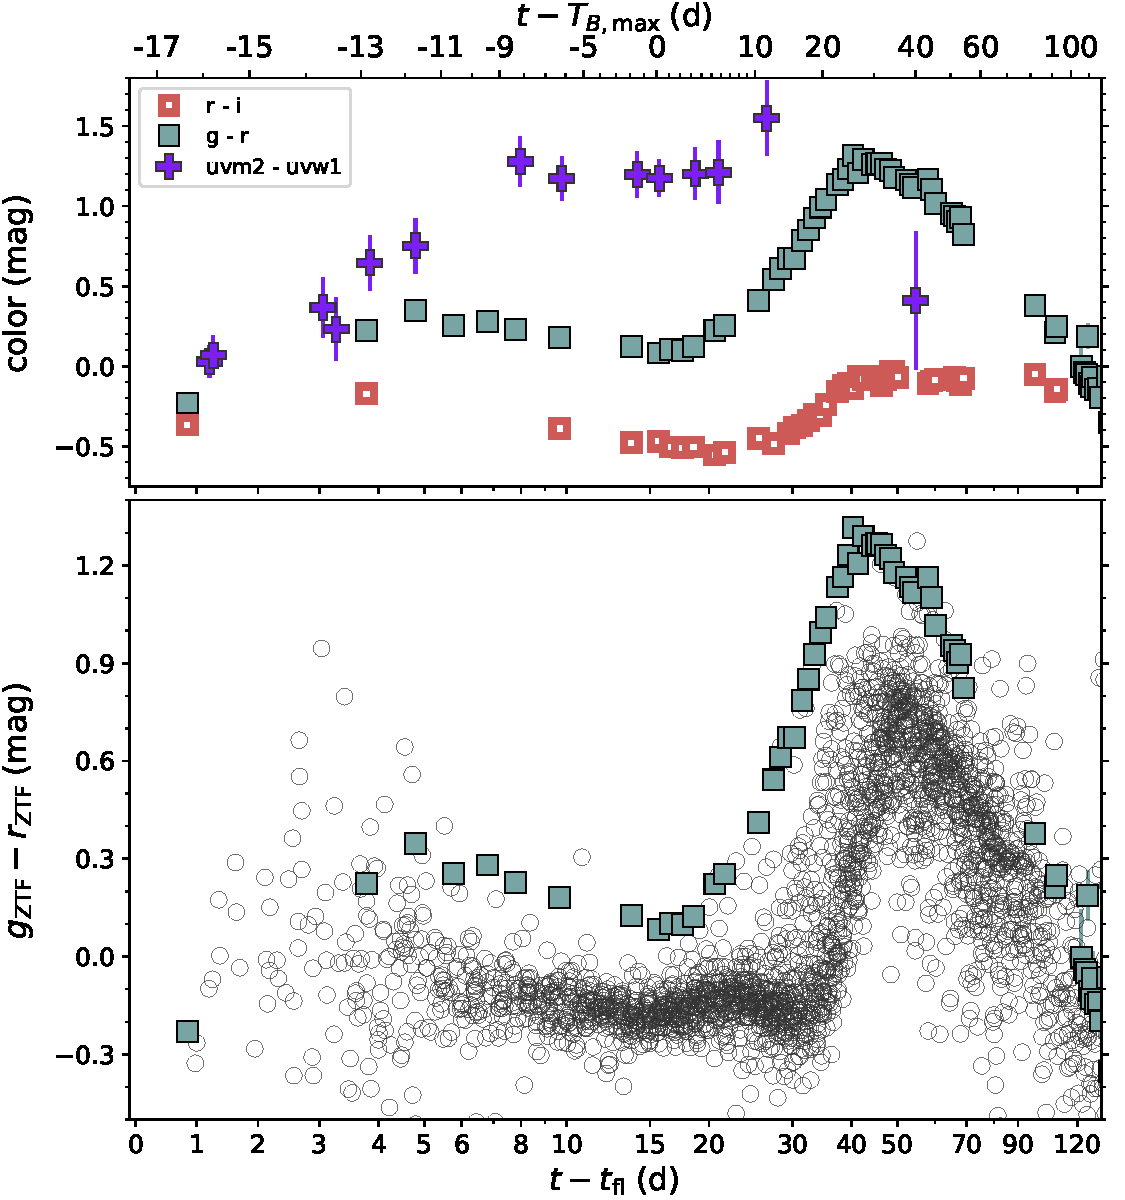
\includegraphics[width=3.35in]{./figures/P48_colors.pdf}
    %
    \caption{Photometric color evolution of \sn. \textit{Top}: \gztf$ -
    $\rztf\ evolution of \sn\ (solid green squares), corrected for the total
    line of sight extinction (see \S\ref{sec:host}), and compared with the
    evolution of 35 normal SNe Ia (open circles) observed within 3\,d of
    \tfl\ by ZTF (from \citealt{Bulla20}). \sn\ is the reddest SN in the
    group, and it exhibits the fastest evolution to red colors post-\tbmax.
    \textit{Bottom}: the $uvm2 - uvw1$ (purple crosses), \gztf$ - $\rztf\
    (solid, green squares), and \rztf$ - $\iztf\ (open, red squares) color
    evolution of \sn. The ``red bump'' can clearly be seen in the
    optical.}
    %
    \label{fig:colors}
\end{figure}

The offset in the \gztf$ - $\rztf\ color evolution of \sn\ relative to normal
SNe\,Ia would be reduced if the reddenning towards \sn\ has been
significantly underestimated. A color excess of $E(B-V) \approx 0.25$\,mag,
rather than the 0.05\,mag adopted in \S\ref{sec:host}, would roughly align
the pre-\tbmax\ \gztf$ - $\rztf\ color of \sn\ with the tight locus seen in
Figure~\ref{fig:colors}. Such a correction would also bring the peak optical
brightness of \sn\ in line with normal SNe\,Ia (for $E(B-V) \approx
0.25$\,mag, $M_g \approx -19.25$\,mag and $M_r \approx -19.1$\,mag for \sn).
Such a large reddening would dramatically change the appearance of \sn\ in
the UV. The bottom panel of Figure~\ref{fig:colors} shows the $uvm2 - uvw1$
color evolution of \sn. At \tbmax, $uvm2 - uvw1 \approx 1.2$\,mag, making
\sn\ one of the most UV blue SNe\,Ia at maximum light (e.g.,
\citealt{Milne10,Brown17}). A color excess of $E(B-V) \approx 0.25$\,mag
would result in $uvm2 - uvw1 \approx 0.7$\,mag at \tbmax, making \sn\ the
most UV blue SN\,Ia observed by \textit{Swift}. Furthermore, this much
extinction would dramatically increase the luminosity of the initial peak in
emission by a factor of $\sim$5. We conservatively estimate the luminosity
$\sim$1.2\,d after \tfl\ to be $\sim$2$\times 10^{42}$\,erg\,s$^{-1}$. It is
difficult to explain such a large luminosity (see below), increasing this by
a factor of 5 and bringing it inline with the typical peak luminosity of
SNe\,Ia, would be nearly impossible to explain. We therefore conclude that
the color excess towards \sn\ is not underestimated, and that the SN is
instead intrinsically red in the optical.

Even if one ignores the striking initial bump in the light curve of \sn, we
can still conclude that \sn\ is not a normal SN Ia based on its other
photometric properties (e.g., low luminosity, fast decline, lack of a
near-infrared secondary maximum, red appearance at peak, and rapid evolution
to red colors after \tbmax).

\todo{discussion of luminosity, teff, etc}

\subsection{Spectral Evolution}\label{sec:spec}

Our initial spectra of \sn\ are dominated by intermediate mass elements
(IMEs), primarily Si, Ca, and O, moving at extremely high velocities ($>
20,000$\,\kms), as identified in Figure~\ref{fig:spec_evo}. In the spectra
obtained $>$10\,d prior to \tbmax, there is also a strong absorption feature
around 4200\,\AA\ that we tentatively identify as \ion{Mg}{II} $\lambda$ 4481.
Though it is also possible that this feature corresponds to the Ti trough
described in \citet{Polin19} for double-detonation SNe Ia. \todo{Could this
feature be \ion{Si}{III}? could explain small notch at ~4500 Ang} While the
early spectra are dominated by IMEs, we find no evidence for \ion{C}{II}
absorption in the spectra of \sn.

Another interesting feature of the early spectra is the relative prominence of
\ion{Si}{II} $\lambda$5972 relative to \ion{Si}{II} $\lambda$6355. Prominent
\ion{Si}{II} $\lambda$5972 absorption suggests a relatively cool photosphere,
however, by the time of maximum light this feature has almost disappeared
entirely. In our maximum-light spectrum of \sn, we estimate pseudo-equivalent
widths (pEWs) of $183\pm1$\,\AA, and $13\pm2$\,\AA\ for \ion{Si}{II}
$\lambda$6355 and $\lambda$5972, respectively. These pEW measurements
unambiguously classify \sn\ as a broad-line SN Ia according to the
classification scheme presented in \citet{Branch06}. The high velocities
typically associated with this class also match the early evolution of \sn.

\begin{figure}
    \centering
    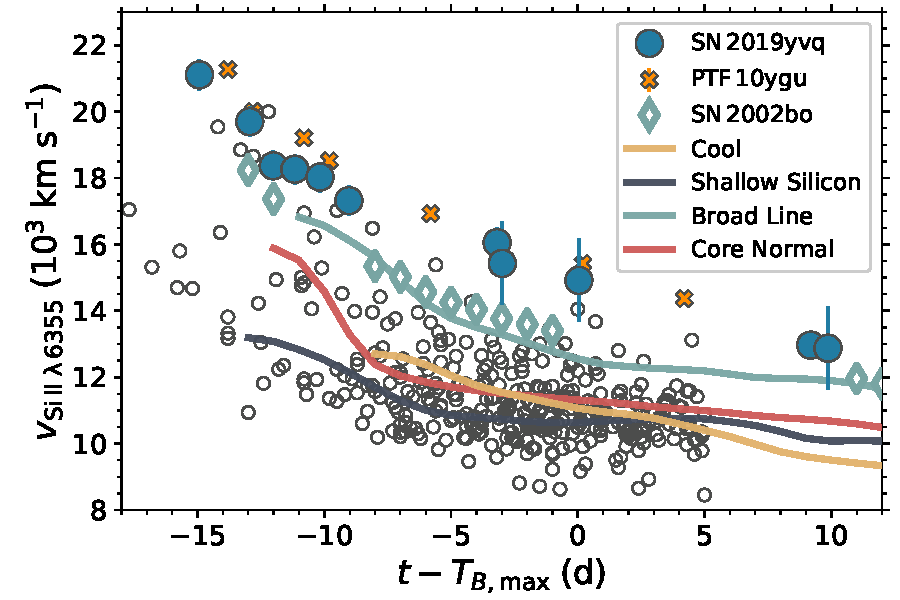
\includegraphics[width=3.35in]{./figures/vel_evolution.pdf}
    %
    \caption{Velocity evolution of \ion{Si}{II} $\lambda$6355\,\AA\ absorption
    in \sn\ (large, filled circles). For comparison we also show the
    measurements for 264 SNe Ia observed by the Palomar Transient Factory
    (PTF) as open circles, with SN\,2010jn (PTF\,10ygu), the SN with the
    fastest moving ejecta in the PTF sample, highlighted via orange crosses.
    We additionally show the velocity evolution of SN\,2002bo, a SN that is
    very similar to \sn, as open diamonds. The median velocity evolution of
    each of the spectroscopic classes defined by \citet{Branch06} (Shallow
    Silicon, Core Normal, Broad Line, and Cool) are shown via solid lines. It
    is clear that \sn\ has exceptionally fast moving ejecta relative to
    typical SNe Ia.}
    %
    \label{fig:vel_evo}
\end{figure}

The velocity evolution of the \ion{Si}{II} $\lambda$6355 absorption feature
in \sn\ is shown in Figure~\ref{fig:vel_evo}. These measurements have been
made following the procedure described in \citet{Maguire14} (see their
\S2.5). For comparison, we also show the \citet{Maguire14} measurements of
the \ion{Si}{II} velocity evolution of 264 SNe Ia observed by the Palomar
Transient Factory (PTF) as open circles in Figure~\ref{fig:vel_evo}, as well
as the median velocity evolution of SNe belonging to the four different
classes (Shallow Silicon, Core Normal, Broad Line, and Cool) identified in
\citet{Branch06}.\footnote{The velocity measurements are from
\citet{Blondin12}, while the method to determine the median velocity is
described in \citet{Miller18}.} \sn\ stands out among other SNe Ia with
some of the highest \ion{Si}{II} velocities that have ever been observed.
Within the PTF sample, only SN\,2010jn exhibits a \ion{Si}{II} absorption
velocity as high as \sn\ at every phase in its evolution. \todo{discuss other
BL with fast Si: sn1997bq , sn2002cd, sn2003W?}

\citet{Benetti04} argue that \ion{S}{II} $\lambda$5640\,\AA, as a weak line,
is more likely to be formed close to the continuum photosphere, and therefore
serves as a better tracer of the photospheric velocity than \ion{Si}{II}
$\lambda$6355\,\AA. We measured the absorption velocity of this line using
the same method described above, and find that the \ion{S}{II} absorption
velocity is remarkably $\sim$3000\,\kms\ slower than \ion{Si}{II}
$\lambda$6355\,\AA\ at all epochs where both features are measurable (from
-12\,d to +0\,d relative to \tbmax). \todo{cut this paragraph?}

In Figure~\ref{fig:r_evo} we show the ratio of the pEW for \ion{Si}{II}
$\lambda$5972\,\AA\ to \ion{Si}{II} $\lambda$6355\,\AA\ [$\equiv
\mathcal{R}($\ion{Si}{II}$)$; see \citealt{Hachinger08} for the updated
definition relative to \citealt{Nugent95}] as a function of time. As first
noted by \citet{Nugent95}, and later confirmed by \citet{Hachinger08},
$\mathcal{R}($\ion{Si}{II}$)$ is a luminosity indicator, with larger values of
$\mathcal{R}($\ion{Si}{II}$)$ corresponding to lower luminosities. 

Shortly after explosion, \sn\ exhibits large values of
$\mathcal{R}($\ion{Si}{II}$)$, yet, by maximum light
$\mathcal{R}($\ion{Si}{II}$)$ declines to low values. Compared to the PTF
spectroscopic sample (\citealt{Maguire14}; open circles in
Figure~\ref{fig:r_evo}), \sn\ has one of the largest values of
$\mathcal{R}($\ion{Si}{II}$)$ after explosion before evoloving to have one of
the lowest values around \tbmax. Qualitatively, this behavior is similar to
SN\,2002bo (open diamonds in Figure~\ref{fig:r_evo}). Such evolution is
atypical, for reference the normal SN\,2011fe is also highlighted in
Figure~\ref{fig:r_evo} (open squares). At face value, the
$\mathcal{R}($\ion{Si}{II}$)$ evolution suggests that the effective
temperature of \sn\ increases significantly as it rises to maximum light. The
optical colors (see Figure~\ref{fig:colors}), however, are nearly constant
throughout this phase while the UV$ - $optical colors clearly decline during
the same period, suggesting a decline in the effective temperature.

\citet{Benetti04} interpret these competing effects as the result of
significant \ion{Si}{II} mixing in the ejecta of SN\,2002bo. Mixing or
producing Si in the outermost layers of the ejecta would (i) lead to larger
\ion{Si}{II} velocities, (ii) produce \ion{Si}{II} line ratios that indicate
cool temperatures (because there is less radioactive material to heat the
ejecta), before eventually (iii) producing low values of
$\mathcal{R}($\ion{Si}{II}$)$ as the photosphere recedes through the ejecta to
higher temperature regions. If this interpretation is correct, this is the
likely explanation for the line ratio evolution seen in \sn. \todo{Does TARDIS
tell us anything about this? I have no idea...} \abi{Any chance this could
somehow be related to burning He to Si in the shell?} \fromkate{Devil's
advocate on this: if the idea is that the outer layers are cooler and the
photosphere recedes then there's no reason why we wouldn't see this effect in
all SNe Ia since all of their velocities decrease with time? }

\begin{figure}
    \centering
    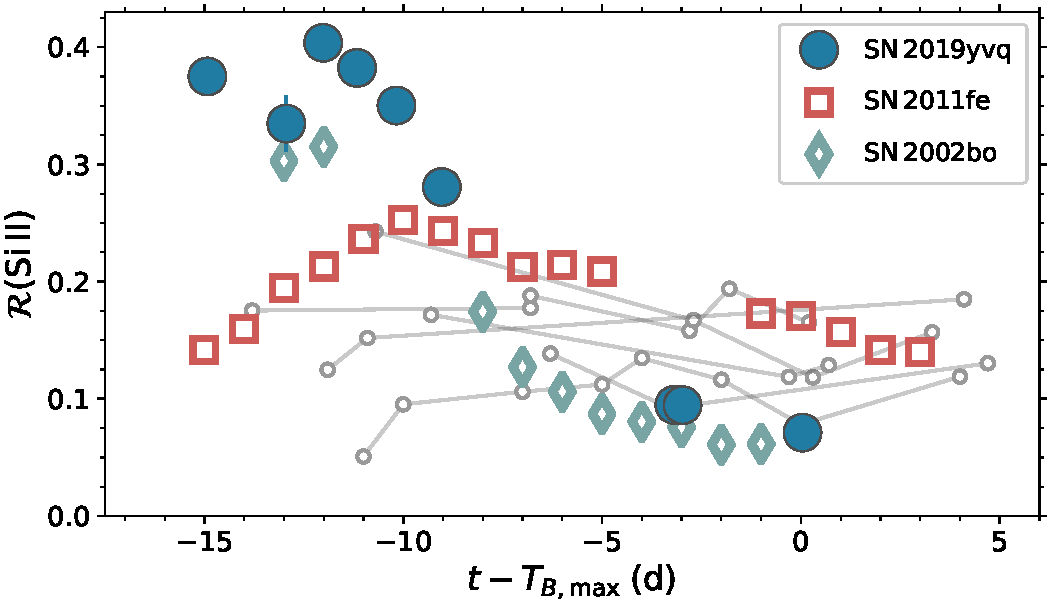
\includegraphics[width=3.35in]{./figures/R_evolution.pdf}
    %
    \caption{Evolution of the ratio of the pEW of \ion{Si}{II}
    $\lambda$5972\,\AA\ to \ion{Si}{II} $\lambda$6355\,\AA,
    $\mathcal{R}($\ion{Si}{II}$)$ in \sn\ (large, filled circles). For
    comparison we also show the measurements for 264 SNe Ia observed by the
    Palomar Transient Factory (PTF) as open circles. The velocity evolution
    of SN\,2002bo and SN\,2011fe are highlighted as open diamonds and open
    squares, respectively. \sn\ and SN\,2002bo exhibit an unusual inversion
    in $\mathcal{R}($\ion{Si}{II}$)$ as they evolve toward maximum light.}
    %
    \label{fig:r_evo}
\end{figure}


\kate{do you want to say anything about \ion{Ca}{II}?}


In Figure~\ref{fig:spec_comp} we compare the spectral evolution of \sn\ to
SN\,2002bo and SN\,2010jn (both \citet{Branch06} Broad Line SNe like \sn).
The evolution of \sn\ and SN\,2002bo is remarkably similar at all phases. The
only significant difference between the two is the absorption trough at
$\sim$4800\,\AA\ in pre- and maximum-light spectra. This feature, which is
typically attributed to a combination of \ion{Fe}{II}, \ion{Fe}{III}, and
\ion{Si}{II}, is extremely narrow in \sn. We believe this is due to a lack of
Fe absorption as the spectra at this epoch show little evidence for iron group
elements (IGEs). SN\,2010jn, which exhibits large \ion{Si}{II} velocities
like \sn, shows weaker IME absorption and stronger IGE absorption than \sn.

\begin{figure*}
    \centering
    \includegraphics[width=7.25in]{./figures/spec_comp.pdf}
    %
    \caption{Spectral comparison of \sn\ to \citet{Branch06} Broad Line and
    Cool SNe\,Ia. \textit{Left panel}: pre-maximum spectra showing the
    similarity of \sn\ and SN\,2002bo. While the expansion velocities in the
    Cool SN\,1986G spectrum are considerably lower than those in the Broad
    Line SNe, the relative ratios of the \ion{Si}{II} features are similar.
    \textit{Second panel}: Comparison of \sn\ to the Broad Line SNe\,2002bo
    and SN\,2010jn. These SNe all feature nearly identical maximum-light
    spectra. By this phase, the relative strength of the \ion{Si}{II}
    absorption features is no longer similar to \citet{Branch06} Cool SNe, as
    illustrated by SN\,2004eo. \textit{Third panel}: $\sim$1 week post-maximum
    spectra. \textit{Fourth panel}: Transitional phase spectra. Comparison
    spectra have been downloaded from WISeREP \citep{Yaron12}, with spectra
    for individual SNe from the following sources: SN\,1986G --
    \citet{Cristiani92}, SN\,2002bo -- \citet{Benetti04,Silverman11},
    SN\,2010jn (PTF\,10ygu) -- \citet{Hachinger13,Maguire14}, SN\,2004eo --
    \citet{Pastorello07}. \todo{Should this be 2 figures?}}
    %
    \label{fig:spec_comp}
\end{figure*}

The left panel of Figure~\ref{fig:spec_comp} also shows the spectrum of
SN\,1986G, a \citet{Branch06} Cool SN that is sometimes referred to as
``transitional'' given its intermediate properties between normal SNe\,Ia and
the sub-luminous SN\,1991bg-like population (e.g., \citealt{Pastorello07}).
The \ion{Si}{II} line ratios, and narrow $\sim$4800\,\AA\ feature in SN\,1986G
are similar to \sn, confirming the cool nature of the photosphere at this
early epoch. The $-12.0$\,d spectrum of \sn\ additionally shows a weaker blue
line in the \ion{S}{II} ``W'' absorption feature at $\sim$5400\,\AA, which is
also consistent with cool temperatures \citep{Nugent95}. \todo{86G had E(B-V)
~ 0.9, correct spectra for that?}

The maximum-light spectra shown in the second panel of
Figure~\ref{fig:spec_comp} reveal much higher temperatures for \sn, as the
\ion{Si}{II} $\lambda$5972\,\AA\ absorption has nearly disappeared by this
epoch. The appearance of \sn, SN\,2002bo, and SN\,2010jn (iPTF\,10ygu) are all
similar at this epoch, with the exception of the 4800\,\AA\ feature mentioned
above. We also show a maximum light spectrum of the \citet{Branch06} Cool,
transitional SN\,2004eo \citep{Pastorello07}. SN\,2004eo has a similar
appearance to \sn, though the lower velocities and cooler temperatures (as
traced by both \ion{Si}{II} $\lambda$5972\,\AA\ and \ion{S}{II}) more clearly
reveal the IGE absorption around 4800\,\AA. \todo{anythingto say about
differences at $\sim$4000\,\AA?}

The third panel of Figure~\ref{fig:spec_comp} shows spectra obtained roughly a
week after maximum light. By this phase absorption due to IGE in \sn\ is
clear. Additional differences between \sn\ and SN\,2002bo can be seen at this
phase. There is stronger absorption in \sn\ blueward of \ion{Ca}{II} H\&K, and
the \ion{S}{II} ``W'' absorption feature is still present in \sn\ and it
cannot be identified in SN\,2002bo or SN\,2010jn. SN\,2004eo maintains an
appearance that is somewhat similar to \sn, though as before, the temperatures
are cooler and the velocities lower.

Spectra obtained $\sim$6 weeks after maximum light are shown in the fourth
panel of Figure~\ref{fig:spec_comp}. At this phase, as the SNe are
transitioning into a nebular appearance, the appearance of each spectrum is
similar modulo some minor differences in the relative line strengths of
different features. \todo{add more discussion here? - I don't know a ton about
this phase of evolution}

\begin{figure*}
    \centering
    \includegraphics[width=6.0in]{./figures/good_model_pl_10.pdf}
    %
    \caption{PRELIMINARY PRELIMINARY PRELIMINARY}
    %
    \label{fig:tardis}
\end{figure*}



\section{A Physical Explanation for \sn}\label{sec:models}

The most striking feature of \sn\ is the observed UV/optical peak that occurs
shortly after discovery (Figure~\ref{fig:p48}). Any model to explain \sn\ must
account for this highly unusual feature. A UV decline in the early phase of a
SN\,Ia has previously only been observed in a single event, iPTF\,14atg
\citep{Cao15}. Resolved ``bumps'' in the early optical emission of SNe\,Ia are
also rare, having only been seen in a few events: SN\,2017cbv
\citep{Hosseinzadeh17} and SN\,2018oh \citep{Shappee19,Dimitriadis19}.
\todo{possibly other cases here, but not ``clearly resolved'' in the way these
two are}

\sn\ features other properties, in addition to an intial peak $\sim$17\,d
prior to \tbmax, that separate it from normal SNe\,Ia. A good model should be
able to explain the following characteristics of \sn:
%
\begin{enumerate}
    \item The early UV/optical ``flash'' (Figure~\ref{fig:p48}).
    \item The low luminosity at maximum light (\S\ref{sec:phot}). 
    \item The rapid optical decline following \tbmax\ (\S\ref{sec:phot}). 
    \item The red optical colors at all epochs (Figure~\ref{fig:colors}). 
    \item The lack of IGE in the early spectra (Figure~\ref{fig:spec_comp}).
    \item The transition from large \RSiII\ values to low values (Figure~\ref{fig:r_evo}).
    \item The large photospheric velocities (Figure~\ref{fig:vel_evo}).
\end{enumerate}
%
As noted in \S\ref{sec:phot}, the photometric evolution of \sn\ is similar to
subluminous 91bg-like SNe, however, the spectra are missing the hallmark
\ion{Ti}{II} absorption trough associated with 91bg-like SNe. Furthermore,
around \tbmax, \RSiII\ is small in \sn, whereas 91bg-like SNe feature large
values of \RSiII\ (e.g., \citealt{Branch09}). Similarly, while the spectral
appearance and evolution of \sn\ is similar to SN\,2002bo, and other
\citeauthor{Branch06} Broad Line SNe, the photometric properties are entirely
different. SN\,2002bo features a relatively slow decline [$\Delta{m}_{15}(B) =
1.13$\,mag] with a clear secondary maximum in the $I$ band \citep{Benetti04},
which is wholey different from what is observed in \sn.

If we otherwise ignore the early flash, the remaining features (2--6) in the
list above can be understood if the explosion that gave rise to \sn\ produced
a relatively small amount of \radni\ that is strongly confined to the inner
regions of the SN ejeta. A low \radni\ yield could explain the underluminous
light curve and red colors, while a highly stratified ejecta structure could
explain the lack of IGE in the early spectra as the IGE would not have been
mixed to these outter layers. Furthermore, with a highly stratified ejecta
composition, the photosphere would transition somewhat rapidly from
\radni-poor to \radni-rich, resulting in a significant change in the
luminosity/temperature of the ejecta along the lines of what we see in the
evolution of \RSiII. \todo{did not explain photospheric velocities}

\citet{Magee20} developed a suite of models featuring different \radni\
structures within the SN ejecta that they then compared to early observations
of SNe\,Ia to see which models replicate what is observed in nature.
Generally, it is found in \citet{Magee20} that highly stratified models do not
match the early evolution of normal SNe\,Ia. However, when we model the early
evolution of \sn\ using the models of \citet{Magee20}, we find that the
observations are best matched by highly stratified models, as shown in
Figure~\ref{fig:Ni_mixing}. For this modelling we have excluded the first two
epochs of ZTF observations, as we consider the mechanism that produces the
early UV flash to be different from the standard \radni\ decay that powers
most SNe\,Ia. That the (normal) rising portion of the \sn\ light curve is best
matched by stratified models strengthens the support for this interpretation.

\begin{figure}
    \centering
    \includegraphics[width=3.35in]{./figures/preliminary_Ni_mixing.png}
    %
    \caption{PRELIMINARY PRELIMINARY PRELIMINARY}
    %
    \label{fig:Ni_mixing}
\end{figure}

On their own, a low-\radni\ yield and highly stratified ejecta fail to explain
the UV/optical flash seen in \sn. A large number of scenarios have been
proposed to explain early ``bumps'' or ``flashes'' in SNe\,Ia light curves,
including: interaction between the SN ejecta and the exploding WD binary
companion \citep{Kasen10a}, interaction between the SN ejecta and
circumstellar material (e.g., \citealt{Dessart14,Piro16}), shock cooling
following the shock breakout from the surface of the WD (e.g.,
\citealt{Piro10,Rabinak11}), double detonation explosions (e.g.,
\citealt{Noebauer17,Polin19}), and extended clumps of \radni\ in the SN ejecta
(e.g., \citealt{Shappee19,Dimitriadis19}). We discuss these models and their
ability to replicate observations of \sn\ below.\footnote{We do not discuss
shock breakout models as our initial detection of \sn\ occurred at $M_g
\approx -16.3$\,mag. A progenitor radius of $\sim$10$\,R_\odot$ is needed to
explain such a high luminosity \citep{Piro10,Rabinak11}, which we consider
implausible for a WD.}

\subsection{Companion Interaction}

For SD progenitors of SNe\,Ia, the SN ejecta will shock on the surface of the
non-degenerate companion giving rise to a short-lived transient in the days
after explosion. \citet{Kasen10a} provided models for the appearance of this
interaction, which is primarily dependent upon the binary separation of the
system (assuming Roche lobe overflow for the non-degenerate companion). The
observed emission following the ejecta-companion collision is dependent upon
the orientation of the system at the time of explosion relative to the line of
sight \citep{Kasen10a}.

An analytic formulation for the luminosity and effective temperature of the
emission from the companion shock is presented in \citet{Kasen10a} (see their
Equations~22 and 25). \citet{Brown12} provide an analytic function to
approximate the fractional decrease in the observed flux as a function of the
orientation of the system. We combine equations from \citet{Kasen10a} and
\citet{Brown12} to model the early emission from \sn\ as ejecta-companion
collision. We assume the interaction emits as a blackbody, and that the
electon scattering opacity $\kappa_e = 0.2$\,cm$^{2}$\,g$^{-1}$ (as in
\citealt{Kasen10a}). Assuming $z_\mathrm{SN} = 0.0094$, $E(B-V)_\mathrm{MW} =
0.018$\,mag, and $E(B-V)_\mathrm{host} = 0.032$\,mag, we compare observed flux
measurements with those predicted by the \citet{Kasen10a} model in epochs with
MJD$\,< 58849.2$ (i.e., the first $\sim$2.5\,d after discovery when emission
from the companion interaction is significantly brighter than the luminosity
due to radioactive decay).\footnote{Given that \sn\ is an unusual SN, we make
no assumptions about the SN emission. The companion-interaction model should
therefore \textit{underestimate} the observed flux as there will be a growing
contribution due to radioactive decay with time.} The model parameters,
including: the companion separation, $a$, the mass of the ejecta,
$M_\mathrm{ej}$, the velocity of the ejecta, $v_\mathrm{ej}$, the angle
between the observer, the SN, and the companion, $\theta$, and the time of
explosion, $t_\mathrm{exp}$ are constrained via a Gaussian likelihood and flat
priors (see Table~\ref{tab:priors}) using an affine-invariant
\citep{Goodman10} Markov Chain Monte Carlo (MCMC) ensemble sampler
\citep{Foreman-Mackey13}.

\begin{figure}
    \centering
    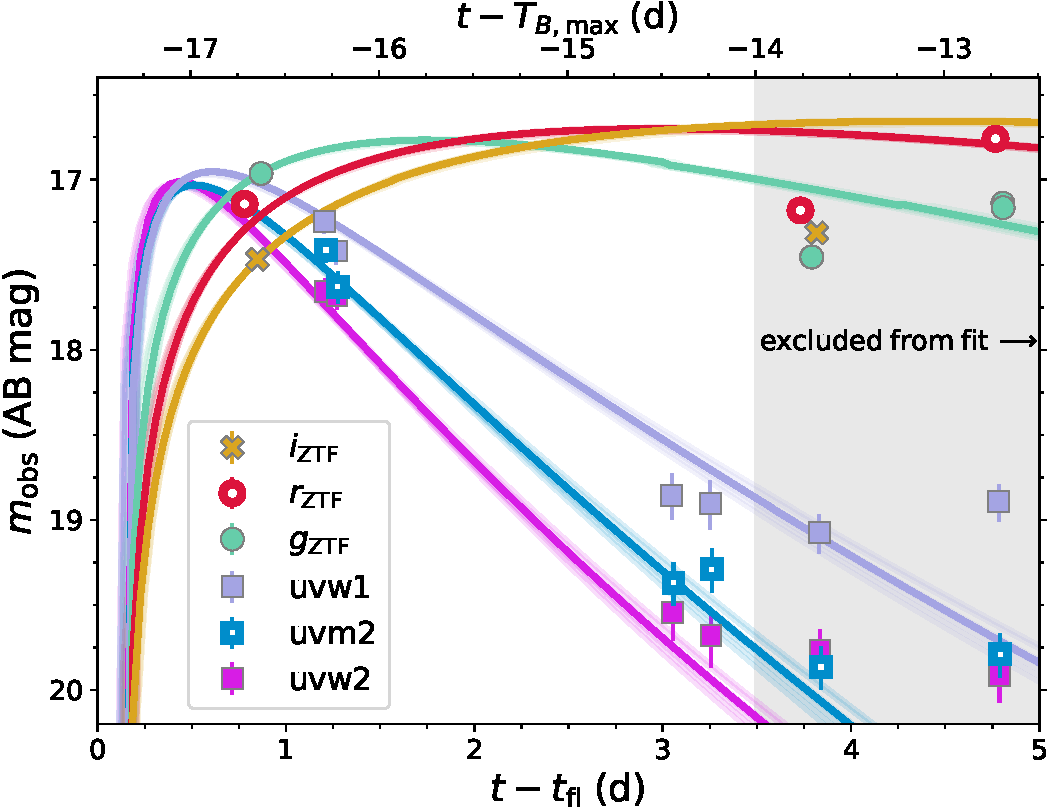
\includegraphics[width=3.35in]{./figures/sn_companion_models.pdf}
    %
    \caption{SN ejecta-companion interaction models compared with the
    UV/optical observations of \sn. Observation symbols are the same as
    Figure~\ref{fig:p48} (solid magenta squares show \textit{Swift} $uvw2$
    observations that are not shown in Figure~\ref{fig:p48}). Solid lines show
    companion interaction model predictions in each filter (the lines have the
    same colors as the corresponding symbols for each passband). The maximum a
    posteriori model is shown via the single bold lines, while other random
    draws from the posterior are shown as thin transparent lines. The shaded
    area shows observations that are excluded from the model fit. The
    overprediction of the optical flux $\sim$13.7\,d prior to \tbmax\ suggests
    that companion interaction does not explain the early flash in \sn\ (see
    text).}
    %
    \label{fig:companion}
\end{figure}

The results of this procedure are shown in Figure~\ref{fig:companion}, where
it is clear that the model presented in \citet{Kasen10a} does an adequate job
of explaining the early UV/optical emission from \sn. We find marginalized
posterior values of $a = 9.1 \pm 0.7 \times 10^{11}$\,cm, $M_\mathrm{ej} = 1.0
\pm 0.3\,M_\odot$, $v_\mathrm{ej} = 2.2 \pm^{0.5}_{0.3} \times 10^{4}$\,\kms,
$\theta = 34 \pm^{28}_{24} \deg$, and $t_\mathrm{exp}(\mathrm{MJD}) = 58845.83
\pm 0.05$ (all uncertainties are 68\% credible regions). Examination of a
corner plot of the posterior samples shows that $M_\mathrm{ej}$ is largely
unconstrained, while $v_\mathrm{ej}$ is degenerate with $\theta$ and $a$ is
degenerate with $t_\mathrm{exp}$. 

While the interaction models roughly approximate the SN emission in the
$\sim$3\,d after explosion, they significantly \textit{overestimate} the flux
immediately after the fitting window as shown in Figure~\ref{fig:companion}.
This problem is exacerbated by the fact that the models do not include
emission associated with radioactive decay, meaning the true discrepancy
between what is predicted and what is observed is even larger than what is
shown in Figure~\ref{fig:companion}. If we extend the fitting window to
include the optical observations obtained $\sim$13.75\,d before \tbmax, the
interaction models still overpredict the optical flux at this epoch. This
overprediction of the optical flux poses a challenge for the companion
interaction scenario; an inability to simultaneously match both UV and optical
observations has been noted for other SNe\,Ia with early bumps or linear rises
\citep{Hosseinzadeh17,Miller18}.

Another challenge for the companion-interaction model is the relatively faint
maximum brightness of \sn. The peak luminosity of a SN\,Ia is directly related
to the total mass of \radni\ synthesized in the explosion \citep{Arnett82},
which is, in turn, correlated with the total ejected mass (see
\citealt{Stritzinger06,Scalzo14,Scalzo14a} and references therein). As an
underluminous explosion, \sn\ likely has a relatively low (i.e.,
sub-Chandrasekhar) $M_\mathrm{ej}$. The companion-interaction model features
systems in Roche-lobe overflow; for H-rich companions thermonuclear runaway
would only be expected as the mass of the WD approaches $M_\mathrm{Ch}$
\todo{REF???}. This is clearly at odds with \sn. Sub-Chandrasekhar explosions
are possible in the double detonation scenario, whereby the WD accretes He
from the companion star. Double detonation explosions can naturally explain
the early UV/optical flash seen in \sn\ (see below), and thus there is no need
to invoke companion interaction in such a scenario. \todo{WHAT DOES EVERYONE
THINK ABOUT THE ARGUMENT IN THIS PARAGRAPH?}
% inferred separation of the companion, $a \approx 9 \times 10^{11}$\,cm.
% Assuming the WD is accreting material via Roche Lobe overflow, then the
% companion radius is $\sim$0.35$a \approx 3.1 \times 10^{11}$\,cm $\approx
% 4.5\,R_\odot$.

For the reasons above, we do not favor the ejecta-companion interaction
interpretation for \sn. \citet{Kasen10a} notes several assumptions and
approximations in the derivation of the equations used to estimate the
emission from the companion shock. It is possible that the inclusion of more
detailed physics, or additional complexity in the analytic formulation of the
models,\footnote{For example, \citet{Kasen10a} points out that the derived
equation for the luminosity of the shock interaction does not account for the
advected luminosity that would be seen in the observer frame.} could better
reconcile companion interaction models with \sn. Such improvements are beyond
the scope of this paper, leading us to explore other explanations for the
early flash.

\subsection{Ni Clumps in the SN Ejecta}

SN\,2018oh was observed with an exquisite 30\,min cadence by the
\textit{Kepler} spacecraft and showed a clearly delineated linear rise in
flux followed by a ``standard'' $t^2$ power-law $\sim$4\,d after \tfl. Models
with extended clumps of \radni\ just below the WD surface have been proposed
as a possible explanation for the initial linear rise in SN\,2018oh
\citep{Shappee19,Dimitriadis19}. The models considered in \citet{Shappee19}
and \citet{Dimitriadis19}, which build on the work of \citet{Piro16}, only
cover the first $\sim$10\,d after explosion and assume relatively simple grey
opacities. To further investigate this possibility, Magee \& Maguire (2020)
recently performed more detailed radiative transfer calculations for SNe\,Ia
with extended clumps of \radni. They then compared these models to SN\,2018oh
and SN\,2017cbv, another event with a clearly resolved bump in the early
light curve \citep{Hosseinzadeh17}.

For \sn\ we follow the procedure in Magee \& Maguire (2020) to model the
early flash and rise of the SN. Briefly, we exclude the first two epochs of
optical detections in ZTF, and identify the best-fit model to the later
evolution of the SN from the grid of models created in \citet{Magee20}.
Following the generation of this ``baseline'' model, we add clumps of \radni\
to the outer layers of the SN ejecta, and perform full radiative transfer
calculations using TURDLS+TARDIS \todo{ref}. We find that a model with
\magee{please add the clump parameters} best matches the optical observations
of \sn, as shown in Figure~\ref{fig:Ni_bullet}. While a clump of \radni\ can
broadly replicate the observed flash in the optical, like Magee \& Maguire
(2020), we find that the extended clump of \radni\ dramatically alters the
appearance of the SN at maximum light in a way that is incompatible with
observed spectra. We therefore conlcude that Ni clumps cannot explain the
early flash seen in \sn.

\begin{figure}
    \centering
    \includegraphics[width=3.35in]{./figures/colour.pdf}
    %
    \caption{PRELIMINARY PRELIMINARY PRELIMINARY}
    %
    \label{fig:Ni_bullet}
\end{figure}

\subsection{Double Detonation Models}

\abi{Best matching double det models}


\section{Rate of Thick He Shell Double Detonation Events}\label{sec:rates}

\textbf{This may not actually be a thick shell}

\aam{Use rough numbers from CLU and simple binomial calculation}

\section{Discussion and Conclusion}\label{sec:conclusions}

\todo{be clever}

\acknowledgements

A.A.M.~is funded by the Large Synoptic Survey Telescope Corporation, the
Brinson Foundation, and the Moore Foundation in support of the LSSTC Data
Science Fellowship Program; he also receives support as a CIERA Fellow by the
CIERA Postdoctoral Fellowship Program (Center for Interdisciplinary
Exploration and Research in Astrophysics, Northwestern University).

This work is based on observations obtained with the Samuel Oschin Telescope
48-inch and the 60-inch Telescope at the Palomar Observatory as part of the
Zwicky Transient Facility project. ZTF is supported by the National Science
Foundation under Grant No. AST-1440341 and a collaboration including Caltech,
IPAC, the Weizmann Institute for Science, the Oskar Klein Center at Stockholm
University, the University of Maryland, the University of Washington,
Deutsches Elektronen-Synchrotron and Humboldt University, Los Alamos National
Laboratories, the TANGO Consortium of Taiwan, the University of Wisconsin at
Milwaukee, and Lawrence Berkeley National Laboratories. Operations are
conducted by COO, IPAC, and UW.

MMT Observatory access was supported by Northwestern University and the
Center for Interdisciplinary Exploration and Research in Astrophysics (CIERA).

We acknowledge the use of public data from the \textit{Swift} data archive.

\software{
          \texttt{astropy} \citep{Astropy-Collaboration13},
          \texttt{scipy} \citep{Jones01}, 
          \texttt{matplotlib} \citep{Hunter07},
          \texttt{pandas} \citep{McKinney10},
        %   \texttt{emcee} \citep{Foreman-Mackey13},
        %   \texttt{corner} \citep{Foreman-Mackey16},
          \texttt{SALT2} \citep{Guy07},
          \texttt{sncosmo} \citep{Barbary16}
          }

%% For this sample we use BibTeX plus aasjournals.bst to generate the
%% the bibliography. The sample63.bib file was populated from ADS. To
%% get the citations to show in the compiled file do the following:
%%
%% pdflatex sample63.tex
%% bibtext sample63
%% pdflatex sample63.tex
%% pdflatex sample63.tex

\bibliography{/Users/adamamiller/Documents/tex_stuff/papers}
\bibliographystyle{aasjournal}

%% This command is needed to show the entire author+affiliation list when
%% the collaboration and author truncation commands are used.  It has to
%% go at the end of the manuscript.
%\allauthors

%% Include this line if you are using the \added, \replaced, \deleted
%% commands to see a summary list of all changes at the end of the article.
%\listofchanges

\begin{deluxetable*}{ccccc}
\tabletypesize{\scriptsize}
\tablewidth{0pt}
\tablecaption{Log of Spectroscopic Observations for SN~2019yvg.\label{tab:spectra}}
\tablehead{
\colhead{Date (UT)}&
\colhead{MJD}&
\colhead{Phase$^{*}$}&
\colhead{Telescope+Instrument}&
\colhead{Range}\\
\colhead{}&
\colhead{(days)}&
\colhead{(days)}&
\colhead{}&
\colhead{(\AA)}}
\startdata
31 Dec 2019 &  58848.273298   &    &  LT+SPRAT$^{*}$ &  4000--9000?   \\
03 Jan 2020 &     &     &  LT+SPRAT$^{*}$ &  4000--9000   \\
04 Jan 2020 &     &     &  LT+SPRAT &  4000--9000   \\
12 Jan 2020 &     &     &  LT+SPRAT &  4000--9000   \\
12 Jan 2020 &     &     &  LT+SPRAT  &  4000--9000   \\
15 Jan 2020 &     &     &  P60+SEDM$^{**}$ &  4000--9000   \\
18 Jan 2020 &     &     &  P60+SEDM &  4000--9000   \\
24 Jan 2020 &     &     &  MMT+Binospec$^{***}$ &  4000--9000   \\
25 Jan 2020 &     &     &  Keck+LRIS$^{****}$ &  4000--9000   \\
27 Jan 2020 &     &     &  P60+SEDM  &  4000--9000   \\
29 Jan 2020 &     &     &  NOT+ALFOSC$^{******}$ &  4000--9000   \\
01 Feb 2020 &     &     &  P60+SEDM &  4000--9000   \\
\enddata
\tablenotetext{*}{Liverpool Telescope}
%\tablenotetext{**}{}
%\tablenotetext{***}{}
\end{deluxetable*}



\end{document}